%\nocite{a565d200}
At the end of section \ref{sec:sset} of chapter \ref{chap:cattg} we quite extensively discussed what the nerve of a covering shall be: something like a sufficiently nice model of a space constructed from a cover capturing homotopy properties of the space. We discussed the traditional notions fitting to what we wanted to say there but we excluded a more modern notion from the discussion which is important for homotopy theory and cohomology in the sense of $(\infty,1)$-topoi: the \textit{\v{C}ech nerve}. We want to make good for this in this section. Yet we will not give a complete discussion on the subject and once more only intend to lead to \cite{a565d200}. On the one hand we lack a precise definition of internal categories and knowledge on simplicial spaces. On the other hand we are not even sure if the following discussion is correct since it seems hard to find good sources on the part of the subject we want to discuss and we didn't have the time yet to explicitly prove the claims ourselves. The discussion is essentially based on
\begin{enumerate}
\item[$\bullet$]
\cite{wiki-pedia0en}: nerve of a covering
\item[$\bullet$]
\cite{wiki-nlab0000}: \v{C}ech methods
\item[$\bullet$]
\cite{wiki-nlab0000}: \v{C}ech nerve
\item[$\bullet$]
\cite{wiki-nlab0000}: \v{C}ech theorem
\end{enumerate}
and how we interpreted these texts. We will start from from the Alexandrov nerve and use {\glqq}simplicial{\grqq} reasoning to find out what the \v{C}ech nerve is. We also try to make clear why it is a good homotopical approximation of the space. Last we will say how we think it can be used to {\glqq}calculate{\grqq} cohomology.
\\\\
So let's start. For the record: we build on section \ref{sec:sset} of chapter \ref{chap:cattg} as if the following would have been written directly below the discussion of the Alexandrov nerve.\footnote{i.p. let $\mathrm{cov}_{S}$ be an open cover generator for the following} We said that traditionally the Alexandrov nerve of some cover is a simplicial complex with $N$-simplices non-empty $N + 1$-fold intersections (up to some technialities). Now note that the intersection of two subsets - and also two open subspaces - is the pullback of one inclusion along the other inclusion as we have discussed in subsection \ref{sec:limit} of chapter \ref{chap:cattg}. But we have already seen that the $N$-simplices for $N \in \mathbb{N}^{\times}$ of the nerve of some (small) category $\mathbf{C}$ are certain fiber products. Namely
\begin{align*}
  \mathrm{n}
  \left(
    \mathbf{C}
  \right)
  ([N])
  &\cong
  \prod_{\mathrm{ob}_{\mathbf{C}}}^{N}
  \mathrm{Mor}_{\mathbf{C}}
\end{align*}
where the latter is the $N$-fold fiber product of the domain function $\mathrm{dom}_{\mathbf{C}}$ and codomain function $\mathrm{cod}_{\mathbf{C}}$. For our purpose this $N$-fold fiber product should be made up by $N+1$-fold non-empty intersections. So we need a category with morphisms corresponding to the $2$-fold non-empty intersections while domain and codomain function should map the the intersection $U_{k_{1}} \cap U_{k_{2}}$ to $U_{k_{1}}$ and $U_{k_{2}}$, respectively. Therefore we need a pullback yielding all $2$-fold non-empty intersections at once. This sounds as if we should consider all inclusions of the cover at once. What we mean is taking the {\glqq}coproduct{\grqq} of all the inclusions. This is to say the unique morphism
\begin{align*}
  \coprod_{k \in K}
  \mathrm{i}_{U_{k}}
  &\in
  \mathrm{mor}_{\mathbf{Set}}
  \left(
    \coprod_{k \in K}
    U_{k},
    S
  \right)
\end{align*}
obtained by universality from the cone consisting of all the $\mathrm{i}_{U_{k}}$ for $k \in K$. Note that this makes also sense in $\mathbf{Top}$ or any category with coproducts. But also note that to make the idea fully sound one should demand a notion of cover for the category such as a Grothendieck topology or so. Anyways let us look what the pullback
\[
\begin{tikzcd}[sep=large]
  \left(
    \coprod_{k \in K}
    U_{k}
  \right)
  \times_{S}
  \left(
    \coprod_{k \in K}
    U_{k}
  \right)
  \arrow{r}{\mathrm{Pr_{2}}}
  \arrow[swap]{d}{\mathrm{Pr_{1}}}
  &
  \coprod_{k \in K}
  U_{k}
  \arrow{d}{\coprod_{k \in K}\mathrm{i}_{U_{k}}}
  \\
  \coprod_{k \in K}
  U_{k}
  \arrow{r}{\coprod_{k \in K}\mathrm{i}_{U_{k}}}
  &
  S
\end{tikzcd}
\]
of
\begin{align*}
  \coprod_{k \in K}
  \mathrm{i}_{U_{k}}
\end{align*}
along itself is. Well, an element of
\begin{align*}
  \coprod_{k \in K}
  U_{k}
\end{align*}
can be regarded as a pair $(x,U_{k})$ for some $k \in K$ such that $x \in U_{k}$. Hence
\begin{align*}
  \left(
    \coprod_{k \in K}
    U_{k}
  \right)
  \times_{S}
  \left(
    \coprod_{k \in K}
    U_{k}
  \right)
\end{align*}
consists precisely of the pairs
\begin{align*}
  \left(
    (x,U_{k_{1}}),
    (x,U_{k_{2}})
  \right)
\end{align*}
where $(x,U_{k_{1}})$ and $(x,U_{k_{2}})$ both correspond to elements of
\begin{align*}
  \coprod_{k \in K}
  U_{k}
\end{align*}
We can consider these as $3$-tuples
\begin{align*}
  \left(
    x,
    U_{k_{1}},
    U_{k_{2}}
  \right)
\end{align*}
by a unique isomorphism from universality of the pullback. These $3$-tuples can be regarded as an ordered formal non-empty intersection of $U_{k_{1}}$ and $U_{k_{2}}$. But we get one for each point in the intersection! And hence taking the nerve of the kernel pair groupoid
\begin{align*}
  \mathbf{G}_{\coprod_{k \in K}\mathrm{i}_{U_{k}}}
\end{align*}
does indeed have ordered $N + 1$-fold intersections as $N$-simplices but one for each point of the intersection. This is a bit too much and we should somehow divide the unnecessary stuff out. But is all the additional stuff really a problem? Not at all we claim. To see what we mean look at
\[
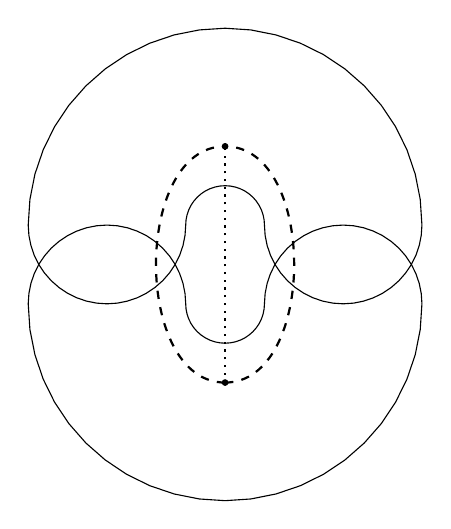
\begin{tikzpicture}[scale=0.5]
  \coordinate (u1) at (0,-3);
  \coordinate (u2) at (0,3);
  \draw[dotted,thick]
    (u1)
    --
    (u2);
  \draw[dashed,thick]
    (u1)
    to[bend left=90]
    (u2);
  \draw[dashed,thick]
    (u1)
    to[bend right=90]
    (u2);
  \draw[domain=0:180]
    plot
    ({cos(\x)},{sin(\x)+1});
  \draw[domain=0:180]
    plot
    ({5*cos(\x)},{5*sin(\x)+1});
  \draw[domain=180:360]
    plot
    ({cos(\x)},{sin(\x)-1});
  \draw[domain=180:360]
    plot
    ({5*cos(\x)},{5*sin(\x)-1});
  \draw[domain=180:360]
    plot
    ({2*cos(\x)-3},{2*sin(\x)+1});
  \draw[domain=180:360]
    plot
    ({2*cos(\x)+3},{2*sin(\x)+1});
  \draw[domain=0:180]
    plot
    ({2*cos(\x)-3},{2*sin(\x)-1});
  \draw[domain=0:180]
    plot
    ({2*cos(\x)+3},{2*sin(\x)-1});
  \filldraw
    (u1)
    circle
    [radius=2pt];
  \filldraw
    (u2)
    circle
    [radius=2pt];
\end{tikzpicture}
\]
The dotted line is what we would traditionally get from an intersection with two path components. But actually it would be closer (it is even the same in this example) to the homotopy type (a circle) of the space covered by these two sets to take an edge for each path component of the intersection with the restriction that they have the same source and target. That is, the two dashed lines. The idea now is to take the neglected topological structure of the coproduct into account. This in particular means that we consider
\begin{align*}
  \coprod_{k \in K}
  \mathrm{i}_{U_{k}}
\end{align*}
as continuous function. Then we call the kernel pair groupoid
\begin{align*}
  \mathbf{G}_{\coprod_{k \in K}\mathrm{i}_{U_{k}}}[\mathbf{Top}]
\end{align*}
internal to $\mathbf{Top}$ the \textbf{\v{C}ech groupoid (for $\mathrm{cov}_{S}$ in $\mathbf{Top}$)}. The internal nerve
\begin{align*}
  \mathrm{n}_{\mathbf{G}_{\coprod_{k \in K}\mathrm{i}_{U_{k}}}[\mathbf{Top}]}
\end{align*}
is called \textbf{\v{C}ech nerve (of $\mathrm{cov}_{S}$ in $\mathbf{Top}$)}. More generally for a category $\mathbf{C}$ with pullbacks and a morphism $f_{12}$ we call the kernel pair groupoid
\begin{align*}
  \mathbf{G}_{f_{12}}[\mathbf{C}]
\end{align*}
the \textbf{\v{C}ech groupoid (for $f_{12}$ in $\mathbf{C}$)} and the internal nerve
\begin{align*}
  \mathrm{n}_{\mathbf{G}_{f_{12}}[\mathbf{C}]}
\end{align*}
the \textbf{\v{C}ech nerve (of $f_{12}$ in $\mathbf{C}$)}. Of course, the case where the domain $X_{1}$ of $f_{12}$ is obtained from something deserving the name {\glqq}cover{\grqq} might be more interesting but it seems that also non-cover cases are interesting or so. But now back to the $\mathbf{Top}$ case. Look at the simplicial space
\begin{align*}
  \mathrm{n}_{\mathbf{G}_{\coprod_{k \in K}\mathrm{i}_{U_{k}}}[\mathbf{Top}]}
\end{align*}
or more specifically at its $N$-simplices
\begin{align*}
  \mathrm{n}_{\mathbf{G}_{\coprod_{k \in K}\mathrm{i}_{U_{k}}}[\mathbf{Top}]}
  ([N])
\end{align*}
which is nothing but a topological space of which we can look at path components. For the sake of simplicity let us only look at the cases $N = 0,1,2$ which actually suffice in the $1$-categorical case. Well,
\begin{align*}
  \mathrm{n}_{\mathbf{G}_{\coprod_{k \in K}\mathrm{i}_{U_{k}}}[\mathbf{Top}]}
  ([0])
  &=
  \mathrm{ob}_{\mathbf{G}_{\coprod_{k \in K}\mathrm{i}_{U_{k}}}[\mathbf{Top}]}
  =
  \coprod_{k \in K}
  U_{k}
\end{align*}
which as set is just the set of pairs $(x,U_{k})$ with $x \in U_{k}$. And the set of path components of $\coprod_{k \in K} U_{k}$ as space is just the set consisting of the path components from all the $U_{k}$. Next look at
\begin{align*}
  \mathrm{n}_{\mathbf{G}_{\coprod_{k \in K}\mathrm{i}_{U_{k}}}[\mathbf{Top}]}
  ([1])
  &=
  \mathrm{Mor}_{\mathbf{G}_{\coprod_{k \in K}\mathrm{i}_{U_{k}}}[\mathbf{Top}]}
  =
  \left(
    \coprod_{k \in K}
    U_{k}
  \right)
  \times_{S}
  \left(
    \coprod_{k \in K}
    U_{k}
  \right)
\end{align*}
which consists of $3$-tuples
\begin{align*}
  \left(
    x,
    U_{k_{1}},
    U_{k_{2}}
  \right)
\end{align*}
such that both $x \in U_{k_{1}}$ and $x \in U_{k_{2}}$. 
\begin{align*}
  \left(
    x,
    U_{k_{1}},
    U_{k_{2}}
  \right)
\end{align*}
and
\begin{align*}
  \left(
    x^{\backprime},
    U_{k_{1}^{\backprime}},
    U_{k_{2}^{\backprime}}
  \right)
\end{align*}
are in the same path component if and only if
\begin{align*}
  U_{k_{1}}
  &=
  U_{k_{1}^{\backprime}}
  \\
  U_{k_{2}}
  &=
  U_{k_{2}^{\backprime}}
\end{align*}
and there is a path from $x$ to $x^{\backprime}$. This follows from the properties of the product, coproduct and subspace topology w.r.t. to path connectedness. This holds more generally in the sense that for some $n \geq 3$
\begin{align*}
  \left(
    x,
    U_{k_{1}},
    \ldots,
    U_{k_{n}}
  \right)
\end{align*}
and
\begin{align*}
  \left(
    x^{\backprime},
    U_{k_{1}^{\backprime}},
    \ldots,
    U_{k_{b}^{\backprime}}
  \right)
\end{align*}
are in the same path component if and only if
\begin{align*}
  U_{k_{1}}
  &=
  U_{k_{1}^{\backprime}}
  \\
  &\cdots
  \\
  U_{k_{n}}
  &=
  U_{k_{n}^{\backprime}}
\end{align*}
and there is a path from $x$ to $x^{\backprime}$. So taking path components of
\begin{align*}
  \mathrm{n}_{\mathbf{G}_{\coprod_{k \in K}\mathrm{i}_{U_{k}}}[\mathbf{Top}]}
\end{align*}
objectwise seems to result in a simplicial set\footnote{this is claimed in \cite{wiki-pedia0en}: nerve of a covering} with one vertex for each path component of the coproduct of all the $U_{k}$, one edge for each path component of each non-empty intersection and so on for higher simplices. Combinatorially, one might object here that one gets two edges for each path component of each non-empty intersection since
\begin{align*}
  \left(
    x,
    U_{k_{1}},
    U_{k_{2}}
  \right)
\end{align*}
and
\begin{align*}
  \left(
    x,
    U_{k_{2}},
    U_{k_{1}}
  \right)
\end{align*}
are not connected by a path and a priori we should fear that we get loops here. But geometrically these should be contractible since as paths in the \v{C}ech groupoid these $3$-tuples are inverse to each other, that is,
\begin{align*}
  \left(
    x,
    U_{k_{1}},
    U_{k_{2}},
    U_{k_{1}}
  \right)
\end{align*}
and
\begin{align*}
  \left(
    x,
    U_{k_{2}},
    U_{k_{1}},
    U_{k_{2}}
  \right)
\end{align*}
are identities. Thus, geometrically, this should not play a role for the homotopy type and we could hope that geometrically realizing the simplicial set obtained from taking objectwise path components of the \v{C}ech nerve of $\mathrm{cov}_{S}$ in $\mathbf{Top}$ is a nice approximation of the space $S$ ideally with the same homotopy type if the space and the cover are good enough. Here we are again at the point of a \textit{nerve theorem}. A version for the Alexandrov nerve seems to be contained in appendix G of chapter 4 of \cite{8b5861fc}. And with some goodwill, arguably the \v{C}ech nerve case, too. Since we assume the internal nerve as internal embedding (motivated from the simplicial set case) we would say that the \v{C}ech groupoid for a good cover is a nice approximation of the homotopy type. What we actually want to drive at is a version of a \v{C}ech groupoid $\check{C}(\lbrace U_{k} \rbrace)$ for a cover $\lbrace U_{k} \rbrace$ of some homotopy type $X$ internal to an $(\infty,1)$-topos ${}_{(\infty,1)}\mathbf{C}$ which is equivalent to $X$ in ${}_{(\infty,1)}\mathbf{C}$ for good covers $\lbrace U_{k} \rbrace$ of the homotopy type $X$. Then to calculate cohomology
\begin{align*}
  {}_{(\infty,1)}\mathbf{C}
  \left(
    X,
    A
  \right)
\end{align*}
it should suffice to determine
\begin{align*}
  {}_{(\infty,1)}\mathbf{C}
  \left(
    \check{C}(\lbrace U_{k} \rbrace),
    A
  \right)
\end{align*}
This seems to be done in \cite{a565d200} using the notion of \textit{$\infty$-anafunctors} which are due to Makkai on the way to a foundation of mathematics by higher category theory. Finally, we can again use \v{C}ech methods in the cohomology classification of $G$-principal bundles in the $(\infty,1)$-topos
 setting in very much the same style as we could in the traditional case. Let us stop here dicussing the \v{C}ech stuff further and just accept the ideas (we hope are correct).
